Tässä luvussa käsitellään ensin työhön keskeisesti kuuluvan verkkoteorian perusteita ja käydään huolellisesti läpi niistä tässä työssä käytettävät osat.
Työssä sovelletaan erityisesti verkkoteorian painotettua verkkoa sekä verkkoteoriassa painotettuihin verkkoihin liittyviä käsitteitä.
Verkkoteoria itsessään on osa diskeettiä matematiikkaa.

Verkkoteorian jälkeen tässä luvussa esitetään vaiheittain työn tuloksena kehitetty priorisointimenetelmä.
Priorisointia varten esitetään harkintaa käyttäen valitut priorisointiin vaikuttavat muuttujat, niitä käyttävät painofunktiot, verkon rakentaminen ja karsiminen sekä verkon ja testitapauksien yhteys.
Lisäksi käydään läpi miten menetelmää käyttäen tuotetun painotetun verkon sisältämää informaatiota voidaan hyödyntää prioriteeteiltaan tärkeimmän polun löytämiseen Dijkstran algoritmia käyttäen.

\section{Matemaattisten verkkojen tarkoitus} \label{ch:09_matemaattisten_verkkojen_tarkoitus}

  Matemaattisten verkkojen tarkoituksena on mallintaa parittaisia riippuvuuksia verkkomaisessa objektijoukossa.
  Verkkoteoriassa peruskäsitteitä ovat itse verkko eli graafi, joka muodostuu solmuista ja niiden välisiä riippuvuuksia esittävistä kaarista tai nuolista.
  Verkkoteorialla on lukuisia käytännön sovellutuksia. Verkkoteoriaa sovelletaan muun muassa tietokonetieteissä, kielitieteissä, fysiikan ja kemian sovellutuksissa, sosiaalisissa tieteissä ja biologiassa.
  Alun perin verkkoteoria katsotaan syntyneen 1700-luvulla esiintyneestä niin sanotusta Königsbergin siltaongelmasta, johon Leonhard Euler esitti todistuksensa \parencite{graph_theory_history}.

  Matemaattisten verkkojen käyttöön päädyttiin tässä työssä siksi, että niiden avulla on hyväksymistestauksen kohteena oleva käyttöliittymä mahdollistaa mallintaa verkoksi.
  Käyttöliittymän verkkomuotoiseen esitykseen voidaan vielä lisätä painot, jotka tässä tapauksessa kuvaavat prioriteetteja, mahdollistaen testikokoelmien priorisoinnin.

\section{Perusmerkinnät ja käsitteet} \label{ch:09_perusmerkinnat_ja_kasitteet}

  Verkkoteoriaa käsittelevässä kirjallisuudessa \parencite{graph_theory_concepts_1}\parencite{graph_theory_concepts_2}\parencite{graph_theory_concepts_3} käytetään muun muassa seuraavia perusmerkintöjä ja käsitteitä:

  \begin{itemize}
    \item \textbf{Solmujoukko} \(V = \{v_a, v_b, v_c\}\) on joukko joka sisältää solmut \(v_a\), \(v_b\) ja \(v_c\).
    \item \textbf{Kaarijoukko} \(E = \{e_{ab}, e_{bc}, e_{ac}\}\) on joukko joka sisältää kaaret \(e_{ab}\), \(e_{bc}\) ja \(e_{ac}\).
    \item \textbf{Verkko} \(G = V(G) \cup E(G)\) on joukko joka sisältää solmujoukon \(V(G)\) ja kaarijoukon \(E(G)\).
    \item \textbf{Aliverkko} \(G_s \subset G\) on verkko \(G_s\) joka koostuu osasta verkon \(G\) solmuja ja kaaria.
    \item \textbf{Polku} \(P = \{v_a, v_b, ..., v_n \: | \: v_a \rightarrow v_n\}\) on solmujono jota pitkin voidaan kulkea solmusta \(v_a\) solmuun \(v_n\).
    \item \textbf{Sykli} \(C = \{v_a, ..., v_n,..., v_a \: | \: v_a \rightarrow v_a\}\) on sellainen polku, jonka aloitussolmu \(v_a\) ja lopetussolmu \(v_a\) ovat sama solmu siten, että polun jokaista kaarta kuljetaan vain kerran.
    \item \textbf{Verkon yhtenäisyys} \(\forall \: v_a \neq v_b \: \exists \: P_{ab}\) tarkoittaa sitä, että \(v_a \rightarrow v_b\), jokaiselle solmuparille on olemassa niitä yhdistävä polku.
    \item \textbf{Solmun asteluku} \(d_G(v_a)\) on solmuun \(v_a\) liittyvien kaarten lukumäärä.
    \item \textbf{Eristetty solmu} on solmu \(v_a\), jonka asteluku on nolla, eli \(d_G(v_a) = 0\).
    \item \textbf{Silta} on solmujen \(v_a\) ja \(v_b\) välinen kaari \(e_{ab}\) siten, että \(d_G(v_a) = 1\) ja \(d_G(v_b) = 1\).
    \item \textbf{Silmukka} on kaari, jonka aloitus- ja lopetussolmu  ovat sama solmu, eli \(v_a \rightarrow v_a\).
  \end{itemize}

\section{Priorisointiin vaikuttavat muuttujat} \label{ch:10_priorisointiin_vaikuttavat_muuttujat}

  Näkymä ja siirtymäperustaiseen priorisointiin vaikuttavat monet eri asiat, joista osa kasvattaa prioriteettia ja osa laskee sitä.
  Prioriteettia kasvattava muuttuja on esimerkiksi liiketoiminnallinen arvo ja laskeva muuttuja on esimerkiksi projektin muutosherkkyys, joka voi johtaa nyt toteutettavien testitapauksien vanhentumiseen tulevaisuudessa.
  Muuttujat ovat kuitenkin hyvin kontekstiriippuvaisia, joten yleispätevää ja kaikkiin tilanteisiin soveltuvaa listaa muuttujista on hankala antaa.
  Kontekstiriippuvaisuuden takia muuttujiin ja myöhemmin esitettäviin painofunktioihin on varattu paikka omille lisämuuttujille.
  Prioriteetin määrittäminen on tässä menetelmässä lineaarista, eli prioriteetti määräytyy sen osiensa summana laskukaavalla joka myöhemmin esitetään.
  Toisin sanoen epälineaarisuutta, eli sellaista tilannetta jossa prioriteettia ei syystä tai toisesta voitaisi ilmoittaa yksinkertaisesti osiensa summana, ei tässä menetelmässä oteta huomioon.

  Tässä diplomityössä esiteltävää priorisointimenetelmää varten jokainen priorisointiin vaikuttava muuttuja arvioidaan asteikolla 1-10, paria poikkeusta lukuun ottamatta.
  Numeerisella asteikolla on tarkoitus antaa korkea numero, jos muuttuja on prioriteetiltaan tärkeä kyseisen näkymän, eli verkon solmun kohdalla.
  Jos jokin muuttuja ei ole kelpoinen siinä kontekstissa, jossa menetelmää yritetään hyödyntää, tulee muuttujan arvo asettaa nollaksi, jolloin se sivuutetaan myöhemmin esitettävässä painofunktiossa.

  Poikkeukselliset muuttujat ovat käyttötapauksien määrä ja siirtymien määrä, joissa numeerisen asteikon sijaan käytetään kyseisten muuttujien määrää suhteessa koko verkkoon.
  Esimerkiksi siirtymien määrää ilmaiseva suhde määritetään laskemalla solmun asteluku \(d_G(v)\), eli solmuun liittyneiden kaarien määrä, jaettuna kaikilla verkossa olevien kaarien määrällä.
  Lisäksi siirtymien määrän suhde vielä kerrotaan luvulla 10, jotta se saadaan skaalautumaan muiden muuttujien kanssa samalle tasolle.

  \begin{table}[H]
    \caption{Näkymä- ja siirtymäperustaiseen priorisointiin vaikuttavat muuttujat}
    \label{tab:priorisointiin_vaikuttavat_muuttujat}
    \centering
    \begin{tabular}{l|l|l|l} \hline
    \(m\) & \textbf{Muuttuja} & \textbf{Etumerkki} & \textbf{Asteikko} \\ \hline
    \textbf{1} & Liiketoiminnallinen arvo & \(+\) & 1 - 10 \\
    \textbf{2} & Liiketoiminnallinen visio & \(+\) & 1 - 10 \\
    \textbf{3} & Negatiivinen käyttäjäpalaute & \(+\) & 1 - 5 \\
    \textbf{4} & Käyttötapauksien määrä & \(+\) & 10 \(\cdot\) suhde  \\
    \textbf{5} & Siirtymien määrä & \(+\) & 10 \(\cdot\) suhde  \\
    \textbf{6} & Positiivinen käyttäjäpalaute & \(-\) & 1 - 5  \\
    \textbf{7} & Muutosherkkyys & \(-\) & 1 - 10  \\
    \textbf{8} & Toteuttamisen kompleksisuus & \(-\) & 1 - 5  \\
    \textbf{9} & Toteutuksen virheherkkyys & \(-\) & 1 - 5  \\
    \textbf{10} & Omat lisämuuttujat & \(\pm\) & 1 - 10 \\ \hline
    \end{tabular}
  \end{table}

\section{Painofunktiot priorisointiin} \label{ch:10_painofunktiot_priorisointiin}

  Painofunktioiden määrittäminen on tärkeä osa painotetun verkon avulla priorisointia, sillä niiden avulla määritetään verkon solmujen ja kaarien prioriteetit.
  Tavanomaisesti numeerinen prioriteetti usein mielletään olevan korkea, jos priorisoitu muuttuja on tärkeä.
  Painotettujen verkkojen tapauksessa on kuitenkin järkevää vaihtaa numeerisen prioriteetin suuntaa, jotta painotettuun verkkoon sovellettavat lyhimmän polun algoritmit toimisivat halutulla tavalla, eli etsien prioriteetiltaan tärkeitä polkuja.

  Ennen prioriteetin suunnanvaihtoa, voidaan kokonaisprioriteetti yksittäiselle solmulle eli näkymälle määrittää kaavalla

  \begin{equation} \label{eq:5_4_1}
    p(v) = \sum\limits_{i=1}^{5} m_i - \sum\limits_{j=6}^{9} m_j \pm m_{10}\text{,}
  \end{equation}

  jossa kokonaisprioriteettia solmulle \(v\) kuvataan funktiona \(p(v)\). Siinä kokonaisprioriteetin arvo määräytyy lineaarisesti osiensa \(m_k\) summana siten, että \(1 \leq k \geq 10\).
  Toisin sanoen prioriteettiin vaikuttavia erilaisia muuttujia on kaavassa yhteensä kymmenen.
  Jokainen kaavassa esiintyvä muuttuja sisältää etumerkin aiemmin esitetyn taulukon \ref{tab:priorisointiin_vaikuttavat_muuttujat} mukaisesti.
  Kaavassa esitetään ensin kokonaisprioriteettiin positiivisesti vaikuttavien muuttujien summa, joka sisältää etumerkiltään positiiviset muuttujat väliltä \(1 \leq i \geq 5\).
  Samalla periaatteella kaavassa esitetään seuraavaksi negatiivisesti vaikuttavat muuttujat väliltä \(6 \leq j \geq 9\), jotka lasketaan ensin yhteen ja vähennetään sitten yhteisesti etumerkillään negatiivisena edellisestä summasta.
  Lopuksi kaavassa on esitetty vielä viimeinen muuttuja \(m_{10}\), joka tarkoittaa taulukon \ref{tab:priorisointiin_vaikuttavat_muuttujat} mukaisesti omaa lisämuuttujaa tai lisämuuttujia, joiden etumerkki voi olla joko positiivinen tai negatiivinen.
  Lisämuuttujien sisällyttämisellä kaavaan on tarkoitus mahdollistaa ja selventää kokonaisprioriteetin laskeminen erilaisissa kontekstiriippuvaisissa tilanteissa sekä osittain myös rohkaista kaikkien prioriteettiin vaikuttavien muuttujien evaluointiin ja muokkaamiseen kontekstista riippuen.

  Prioriteetin suunnan vaihtamiseksi suuresta pieneen, säilyttäen kuitenkin prioriteetin sisältämän informaation, voi hoitaa käänteislukujen avulla.
  Ennen käänteisluvuksi muuttamista, prioriteettiin vaikuttavien muuttujien yhteenlaskettu summa voi olla ongelmallisesti negatiivinen tai nolla.
  Negatiiviset arvot eivät ole painotetun verkon kannalta erityisen järkeviä, sillä tässä diplomityössä hyödynnettävää Dijkstran algoritmia ei voida käyttää negatiivisien painojen kanssa.
  Dijkstran algoritmin toiminta nollan tapauksessa voi myös kuulostaa epäilyttävältä, kuten esimerkiksi tilanne, jossa painotetun verkon kaikki painot olisivat nollia.
  Dijkstran algoritmin tapauksessa tällainen verkko on kuitenkin sallittu, koska silloin lyhimmän polun ratkaisu on verkon kaikki solmut.
  Lyhimmän polun ongelman erityisvaatimusten lisäksi käänteislukua varten nolla on huono arvo siinä mielessä, että sille ei ole olemassa lainkaan käänteislukua.
  Tämä johtuu siitä, että jos nollalle yrittäisi etsiä käänteislukua, tulisi eteen nollalla jakaminen jota ei voi tehdä.
  Nämä molemmat ongelmatapaukset voidaan kuitenkin painofunktioissa ratkaista siten, että käänteisfunktiota ei etsitä, vaan korvataan painofunktion tulos yhdellä.

  Painofunktio yksittäiselle solmulle \(v\), eli näkymälle saadaan solmun kokonaisprioriteetin \(p(v)\) käänteislukuna kaavalla

  \begin{equation} \label{eq:5_4_2}
    \alpha(v) = \begin{cases}
      p^{-1}(v) & p(v) > 0 \\
      1 & p(v) \leq 0
    \end{cases}
    \text{,}
  \end{equation}

  jossa solmun \(v\) käännettyä kokonaisprioriteettia kuvataan funktiona \(\alpha(v)\).
  Solmun kokonaisprioriteettia vastaava käänteisluku etsitään vain siinä tapauksessa jos kokonaisprioriteetti on suurempi kuin nolla.
  Jos vastaan tulee tilanne, jossa kokonaisprioriteetti olisi negatiivinen tai yhtä suuri kuin nolla ei käänteislukua yritetä ottaa vaan tulos korvataan suoraan käännettyjen prioriteettien alhaisimmalla arvolla, eli luvulla yksi.
  Toisin sanoen painofunktiosta saatava numeerinen arvo tarkoittaa käytännössä sitä, että mitä pienempi se on sitä korkeampaa prioriteettia se edustaa.

  Painofunktio yksittäiselle kaarelle \(e_{ab}\) eli solmuja \(v_a\) ja \(v_b\) yhdistävälle käyttöliittymän näkymien väliselle siirtymälle saadaan kaavalla

  \begin{equation} \label{eq:5_4_3}
    \beta(e_{ab}) = \begin{cases}
      [p(v_a) + p(v_b)]^{-1} & p(v_a) + p(v_b) > 0 \\
      1 & p(v_a) + p(v_b) \leq 0
    \end{cases}
    \text{,}
  \end{equation}

  jossa kaaren \(e_{ab}\) käännettyä kokonaisprioriteettia kuvataan funktiona \(\beta(e_{ab})\). Kaaren painofunktiota varten pitää kuitenkin huomioida, että sen kokonaisprioriteetti on kaaren päätepisteiden, eli aloitus- ja lopetussolmujen kokonaisprioriteetin summa \(p(v_a) + p(v_b)\).
  Kaaren kokonaisprioriteetti pitää siis laskea ennen käänteisluvuksi muuttamista.
  Kaaren painofunktioon \(\beta(e)\) pätee samat reunaehdot kuin yksittäisen solmun painofunktioonkin \(\alpha(v)\).

\section{Verkon rakentaminen} \label{ch:10_verkon_rakentaminen}

  Tässä diplomityössä on aiemmin moneen otteeseen kerrottu näkymä ja siirtymäperusteisesta testiautomaation toteuttamisesta ja priorisoinnista.
  Painotetun verkon rakentamista varten tulee tarvittavat näkymät ja niiden väliset siirtymät muodostavat testauskohteen käyttöliittymästä.
  Web-sovelluksen käyttöliittymän näkymiä ovat muun muassa sivut, sivujen sisältämät säiliö-elementit ja dialogit.
  Jos käyttöliittymän näkymä sisältää tilan, eli kyseinen näkymä muuttuu käyttäjän tekemien toimenpiteiden perusteella, käsitellään kyseinen tilallinen näkymä painotetussa verkossa kuitenkin yhtenä solmuna.
  Tällaisessa tapauksessa menetelmän käyttö priorisoi kyseisen näkymän joka periaatteessa vastaa sellaista testikokoelmaa, johon rakennettaisiin testitapaukset eri tilanteita varten.
  Siirtymät ovat usein sivujen välisiä linkkejä tai vaihtoehtoisesti jotakin sellaista toiminnallisuutta, joka muuttaa nykyisen näkymän tai osan siitä toiseksi näkymäksi.

  Seuraavassa taulukossa \ref{tab:esimerkki_verkon_priorisointi_muuttujat} on esitetty kuvitteellisen web-sovelluksen mukainen näkymien ja siirtymien mukaan laadittu esimerkki.
  Taulukossa esitetään näkymät kirjautumisnäkymästä ohjenäkymään ja jokaisen näkymän siirtymät eli yhteydet toisiin näkymiin.
  Näkymät ja siirtymät luovat matemaattisen verkon laatimisen perusedellytykset, eli datan jonka avulla myöhemmin esitettävä painomatriisi voidaan laatia.
  Taulukossa on lisäksi esitetty jokainen näkymään liittyvä priorisointiin vaikuttava muuttuja.
  Priorisointiin vaikuttavien muuttujien arvot on laadittu subjektiivisesti kuvitteellisen esimerkin muodossa.
  Priorisointiin vaikuttavien muuttujien yhteenlaskettu prioriteetti yksittäiselle näkymälle on laskettu taulukkoon valmiiksi käyttäen aiemmin esitettyä prioriteettifunktiota \(p(n)\), jossa \(n\) tarkoittaa sitä näkymää jolle prioriteetti lasketaan.

  \begin{table}[H]
    \caption{Esimerkkiverkon näkymät, siirtymät ja priorisointimuuttujat}
    \label{tab:esimerkki_verkon_priorisointi_muuttujat}
    \centering
    \begin{tabular}{l|l|l|l|l|l|l|l|l|l|l|l|l} \hline
    \(n\) & \textbf{Näkymä} & \textbf{Siirtymät} & \(m_1\) & \(m_2\) & \(m_3\) & \(m_4\) & \(m_5\) & \(m_6\) & \(m_7\) & \(m_8\) & \(m_9\) & \(p(n)\) \\ \hline
    \textbf{A} & Kirjautuminen & B & 10 & 10 & 0 & 2 & 1 & 0 & 5 & 5 & 5 & 8 \\
    \textbf{B} & Pelivalikko & A, C, D, G & 8 & 10 & 1 & 2 & 4 & 4 & 5 & 5 & 5 & 6 \\
    \textbf{C} & Asetukset & A, B & 4 & 6 & 5 & 2 & 2 & 2 & 5 & 5 & 5 & 2 \\
    \textbf{D} & Peli & B, E, G & 10 & 10 & 4 & 2 & 3 & 4 & 4 & 5 & 5 & 11 \\
    \textbf{E} & Tulokset & B, D, F & 6 & 8 & 0 & 2 & 3 & 5 & 5 & 4 & 5 & 2 \\
    \textbf{F} & Onnittelu & B, E & 1 & 8 & 0 & 0 & 2 & 2 & 5 & 2 & 5 & -3 \\
    \textbf{G} & Ohje & B, D & 1 & 10 & 2 & 0 & 2 & 0 & 8 & 0 & 0 & 7 \\ \hline
    \end{tabular}
  \end{table}

  Painotetun verkon rakentamisen syötteeksi täytyy käyttöliittymän näkymät ja siirtymät sekä niiden painoarvot esittää painomatriisin muodossa.
  Painoarvot saadaan aiemmin esitetyn painofunktion \(\beta(e)\) avulla.
  Painoarvo lasketaan kyseisen funktion avulla jokaiselle kahta näkymää yhdistävälle siirtymälle, eli painotetun verkon solmujen väliselle kaarelle.
  Painofunktio \(\beta(e)\) käyttää kaaren molempien päätepisteiden yhteenlaskettua prioriteettia, josta käänteisluku otetaan.
  Näin saadaan laskettua kaarelle sellainen painoarvo, joka tarkoittaa painotetussa verkossa siirtymän näkymiin sidottua prioriteettia.
  Esimerkkinä voidaan laskea taulukon \ref{tab:esimerkki_verkon_priorisointi_muuttujat} mukaisten näkymien \(v_a\) ja \(v_b\) välisen siirtymän, eli kaaren \(e_{ab}\) painoarvo \(\beta(e_{ab})\) seuraavalla laskutoimituksella

  \begin{equation} \label{eq:5_5_1}
    \beta(e_{ab}) = [p(v_a) + p(v_b)]^{-1} = (8 + 6)^{-1} = \frac{1}{14} \approx 0.071
    \text{.}
  \end{equation}

  Painofunktioiden lisäksi painotetun verkon esittämistä varten tarvitaan painomatriiseja.
  Painomatriisin avulla voidaan rakentaa matemaattinen painotettu verkko, joka kuvaa näkymiä ja siirtymiä sekä niiden prioriteetteja.
  Painomatriiseissa tulee lähes väistämättä esiin tilanne, jossa pitäisi määrittää painoarvo olemattomalle silmukalle, eli kaarelle jonka aloitussolmu ja lopetussolmu ovat sama solmu itsessään, mutta kaarta ei ole olemassa.
  Tällaisissa tapauksissa, tilanteesta riippuen painomatriiseihin usein merkitään \(0\), \(\infty\) tai \(-\) \parencite{graph_theory_concepts_1}.
  Tässä diplomityössä esitettävän menetelmän painomatriiseissa solmuun itseensä johtuvan kaaren, eli silmukan painoksi merkitään aina \(-\), koska käyttöliittymän näkymästä siirtymät itseensä ei tässä menetelmässä käsitellä varsinaisina siirtyminä.
  Tämän lisäksi luonnollisesti jokainen sellainen solmupari, jolla ei ole niitä yhdistävää kaarta merkitään painomatriisiin käyttäen \(-\) merkintää.
  Sellaisien siirtymien toiminnallisuuden testaaminen on tarkoitus kattaa näkymän mukaisen testikokelman testitapauksissa ja ne tulee priorisoiduiksi näkymä- ja siirtymäperusteisesti.
  Painotetun verkon kaaret voivat verkkoteorian mukaan olla suunnattuja tai suuntaamattomia.
  Tässä esimerkkitapauksessa jokainen siirtymä näkymien välillä on suuntaamaton, eli toisin sanoen käyttöliittymässä kaksisuuntainen ja se priorisoidaan sen mukaisesti.
  Painomatriisissa suuntaamattomien kaarien johdosta voidaan huomata, että painomatriisin diagonaalin erottamat puoliskot ovat toistensa peilikuvia.
  Painomatriisi taulukon \ref{tab:esimerkki_verkon_priorisointi_muuttujat} mukaiselle esimerkille ja siitä lasketuille painoarvoille on pyöristettynä kolmen desimaalin tarkkuudelle seuraavanlainen

  \begin{equation} \label{eq:5_5_2}
    M_G \approx
    \bordermatrix{
      G   & v_a   & v_b   & v_c   & v_d   & v_e   & v_f   & v_g   \cr
      v_a & -     & 0.071 & 0.100 & -     & -     & -     & -     \cr
      v_b & 0.071 & -     & 0.125 & 0.059 & 0.125 & 0.333 & 1.000 \cr
      v_c & 0.100 & 0.125 & -     & -     & -     & -     & -     \cr
      v_d & -     & 0.059 & -     & -     & 0.077 & -     & 0.250 \cr
      v_e & -     & 0.125 & -     & 0.077 & -     & 1.000 & -     \cr
      v_f & -     & 0.333 & -     & -     & 1.000 & -     & -     \cr
      v_g & -     & 1.000 & -     & 0.250 & -     & -     & -     \cr
    }
    \text{.}
  \end{equation}

  Painomatriisin määrittämisen jälkeen voidaan edetä painotetun verkon kuvaamiseen, jossa piirretään jokainen erilaista käyttöliittymän näkymää vastaava, esimerkkidatan mukainen solmu ja niiden välisiä siirtymiä kuvaavat yhteydet eli kaaret.
  Kaarien yhteyteen lisätään painomatriisista kaaren prioriteettia kuvaava painoarvo.
  Seuraavassa on esitetty painomatriisia vastaava painotetun verkon kuvaaja sellaisena kuin se on ennen siihen tehtäviä prioriteettileikkauksia.
  Toisin sanoen kyseinen painotetun verkon kuvaaja on lähtötilanne, josta priorisointi aloitetaan.
  Priorisoimista varten tehtävien leikkauksien tekeminen niitä varten kehitetyllä toistettavalla karsimisalgoritmilla esitetään myöhemmin omassa kappaleessaan.

  \begin{figure}[H]
    \centering
    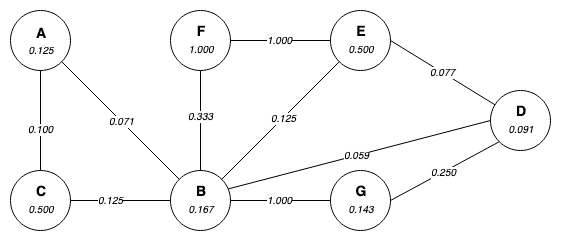
\includegraphics[width=0.8\textwidth]{assets/painotettu-verkko-ennen.png}
    \caption{Esimerkki painotetusta verkosta ennen leikkauksia}
    \label{fig:painotettu-verkko-ennen}
  \end{figure}

  Perinteisesti painotetuissa verkoissa ei esitetä yksittäisiä solmupainoja vaan painotetun verkon painoilla tarkoitetaan solmujen välisien kaarien painoarvoja.
  Tässä diplomityössä kehitettyä menetelmää käytettäessä edellä esitettyyn painotettuun verkkoon on kuitenkin lisätty painomatriisin sisältämän informaation lisäksi painofunktion \(\alpha(v)\) avulla lasketut yksittäisten solmujen eli näkymien painoarvot.
  Esimerkkinä voidaan laskea taulukon \ref{tab:esimerkki_verkon_priorisointi_muuttujat} mukaisen näkymän eli solmun \(v_a\) painoarvo \(\alpha(v_a)\) seuraavalla laskutoimituksella

  \begin{equation} \label{eq:5_5_3}
    \alpha(v_a) = p^{-1}(v_a) = 8^{-1}  = 0.125
    \text{.}
  \end{equation}

  Yksittäisten solmujen prioriteettia kuvaavat painoarvot ovat erittäin merkittäviä ja hyödyllisiä, sillä niiden avulla voidaan järjestää itse solmut, eli näkymät prioriteettien mukaiseen järjestykseen.
  Tämän lisäksi solmujen prioriteettien avulla voidaan verkkoon muun muassa soveltaa lyhimmän polun ratkaisemiseen kehitettyjä algoritmeja, kuten myöhemmin Dijkstran algoritmin osalta esitetään omassa kappaleessaan.

\section{Verkon karsiminen} \label{ch:10_verkon_karsiminen}

  Painotetun verkon karsiminen eli sen kaarien leikkaaminen on yksi prioriteeillä painotetun verkon erittäin tärkeä ominaisuus.
  Verkkoteorian soveltaminen prioriteettien avulla painotettuun verkkoon on erityisen hyödyllistä silloin, kun verkon kaarissa alhainen paino tarkoittaa suurta prioriteettia.
  Tässä diplomityössä verkon karsiminen tapahtuu varta vasten kehitetyllä kolmivaiheisella iteratiivisesti toistettavalla algoritmilla, jonka käyttämistä varten valitaan ensin kattavuus joka vastaa sitä minimirajaa jonka jälkeen karsiminen lopetetaan.
  Kattavuus tarkoittaa samalla myös testikattavuutta testikokoelmien näkökulmasta, sillä painotetussa verkossa jokainen solmu eli näkymä voidaan ajatella vastaavan sen mukaan kategorisoitua testikokoelmaa.

  Verkkoon tehtäviä leikkauksia varten määritettävä kattavuus \(c\) on prosentuaalinen raja sille kuinka suuri osa verkon solmuista eli näkymistä täytyy verkkoon jäädä karsimisen jälkeen.
  Leikkauksien tekemistä suoritetaan toistuvasti niin kauan, kuin karsittavan verkon solmujen lukumäärä on suurempi, mitä kattavuuden määräämä alaraja sallii, tai jos kyseisellä iteraatiokerralla ei yksinkertaisesti enää löydy algoritmiin kuuluvilla toimenpiteillä poistettavia solmuja.
  Matemaattiseen muotoon kirjoitettuna kattavuuteen perustuva toistamisen lopettava ehto on

  \begin{equation} \label{eq:5_6_1}
    |V(G_s)| >  \frac{c}{100} \cdot |V(G)|
    \text{,}
  \end{equation}

  jossa \(|V(G_s)|\) tarkoittaa karsitun verkon solmujoukon mahtavuutta, ja vastaavasti  \(|V(G)|\) tarkoittaa alkuperäisen verkon solmujoukon mahtavuutta eli solmujen lukumäärää.
  Ehto voidaan myös ajatella yksinkertaisesti aliverkon solmujen lukumääränä, jonka täytyy olla suurempi kuin muuttujan \(c\) mukainen prosentuaalinen osuus alkuperäisen verkon solmujen lukumäärästä.
  Tässä verkon karsimisen esimerkissä kattavuutena käytetään \(c = 80\), joka tarkoittaa esimerkkiverkon alkuperäisten solmujen määrän \(7\) karsimista määrään \(80 \cdot \frac{7}{100} = 5.6\), eli lukumäärään \(5\) asti.

  Algoritmissa on kolme erilaista toimenpidettä verkon karsimiseen.
  Toimenpiteillä on suoritusjärjestys, jonka mukaan kyseisellä iteraatiokerralla tehtävä leikkaus määräytyy.
  Jokaisella toimenpiteellä on myös oma suoritusehto, jonka täytyy täyttyä ennen kyseisen toimenpiteen suorittamista.
  Suoritusjärjestyksen ja ehtojen perusteella siirrytään toimenpiteestä toiseen yhden iteraatiokerran aikana siten, että jos esimerkiksi ensimmäistä toimenpidettä ei sen suoritusehdon mukaan voida tehdä yritetään suorittaa toimenpiteistä seuraavaa.
  Jokaisella iteraatiokerralla suoritetaan vain yksi toimenpide, jonka jälkeen aloitetaan uusi iteraatiokierros.
  Algoritmiin sisältyy seuraavat toimenpiteet niiden oikeaan suoritusjärjestykseen järjestettynä.

  \begin{enumerate}
    \itemsep1em
    \item \textbf{Poistetaan verkosta löytyvä eristetty solmu} eli solmu jonka asteluku on nolla.
    Eristettyjä solmuja ei alkuperäisestä verkosta pitäisi löytyä lainkaan, vaan ne ovat seurausta eri iteraatiokerroilla tapahtuneista leikkauksista.
    Toimenpiteen suoritusehto on muotoa
      \begin{equation} \label{eq:5_6_2}
        d_G(v) = 0
        \text{,}
      \end{equation}
    jossa \(d_G(v)\) tarkoittaa astelukua  kuvaavaa funktiota solmulle \(v\).
    \item \textbf{Poistetaan verkosta löytyvä sillattu solmu} leikkaamalla siihen liittyvä kaari.
    Solmun asteluvun täytyy olla yksi ja sen painon pienempi kuin alkuperäisen verkon solmujen painojen keskiarvo.
    Toimenpiteen suoritusehto on kaksiosainen ja muotoa
      \begin{equation} \label{eq:5_6_3}
        d_G(v) = 1 \;\; \land \;\; \alpha(v) < \frac{1}{|V(G)|} \cdot \sum\limits_{v \in V(G)} \alpha(v)
        \text{,}
      \end{equation}
    jossa \(d_G(v)\) tarkoittaa astelukua solmulle \(v\) ja \(|V(G)|\) tarkoittaa alkuperäisen verkon solmujen lukumäärää sekä \(\sum\limits_{v \in V(G)} \alpha(v)\) tarkoittaa alkuperäisen verkon solmujen painoarvojen yhteenlaskettua summaa.
    \item \textbf{Poistetaan verkosta solmu, jolla on maksimia pienempi asteluku ja keskimääräistä pienempi paino.}
    Toisin sanoen poistetaan verkosta sellainen alhaisimman prioriteetin solmu, jonka asteluku on pienempi kuin solmujen astelukujen keskiarvo ja sen paino on pienempi kuin alkuperäisen verkon solmujen painojen keskiarvo.
    Toimenpiteen suoritusehto on kaksiosainen ja muotoa
      \begin{equation} \label{eq:5_6_4}
        d_G(v) < \text{max}\{d_G(x) | x \in V(G)\} \;\; \land \;\; \alpha(v) < \frac{1}{|V(G)|} \cdot \sum\limits_{v \in V(G)} \alpha(v)
        \text{,}
      \end{equation}
    jossa \(d_G(v)\) tarkoittaa astelukua solmulle \(v\) ja \( \text{max}\{d_G(x) | x \in V(G)\}\) tarkoittaa maksimia alkuperäisen verkon solmujen asteluvuista.
    Keskiarvon laskemiseen liittyvät merkinnät \(|V(G)|\) ja \(\sum\limits_{v \in V(G)} \alpha(v)\) ovat samat kuin edeltävässäkin toimenpiteessä.
  \end{enumerate}

  Tässä diplomityössä läpikäytävässä taulukon \ref{tab:esimerkki_verkon_priorisointi_muuttujat} mukaisessa verkon karsimisen esimerkissä algoritmia suoritetaan kaksi iteraatiokierrosta.
  Kahden iteraatiokierroksen jälkeen verkon solmujen määrä karsiutuu prioriteettien ja valitun kattavuuden \(c=80\) mukaisesti seitsemästä viiteen.

  \begin{figure}[H]
    \centering
    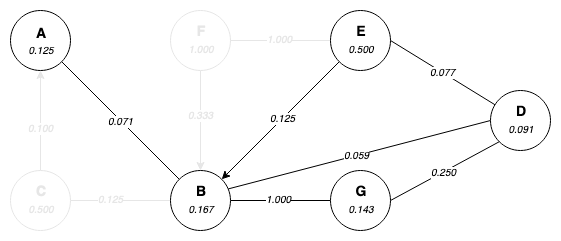
\includegraphics[width=0.8\textwidth]{assets/painotettu-verkko-jalkeen.png}
    \caption{Esimerkki painotetusta verkosta leikkauksien jälkeen}
    \label{fig:painotettu-verkko-jalkeen}
  \end{figure}

  Verkon karsimisen jälkeen voidaan huomata, että verkosta on karsiutunut pois kaksi prioriteeteiltaan alhaisinta solmua C ja F.
  Lisäksi alkuperäisestä verkosta \ref{fig:painotettu-verkko-ennen} voidaan huomata, että solmuilla C ja E olisi keskenään yhtä suuri prioriteetti, mutta asteluvuiltaan ne ovat erilaiset.
  Algoritmi toimii kyseisessä tapauksessa oikein ja karsii edellä mainituista solmuista solmun C.
  Esimerkin mukaisen solmujen karsimisen myötä voidaan todeta, että algoritmi toimii siten kuin sen kuuluukin.

\section{Dijkstran algoritmin hyödyntäminen} \label{ch:10_dijkstran_algoritmin_hyodyntaminen}

  Priorisointimenetelmän mukaan karsittuun painotettuun verkkoon on mahdollista soveltaa lyhimmän polun ongelman ratkaisemiseen kehitettyjä algoritmeja.
  Ne toimivat normaaliin tapaan etsien numeerisesti alhaisimman painoarvon polkuja, joka kuitenkin tässä menetelmässä tarkoittaa käänteisesti korkeimman prioriteetin polkuja.
  Lyhimmän polun etsimiseen on tarkoitus valita sellaiset aloitus- ja lopetussolmut, joiden välille lyhin polku verkossa halutaan etsiä.
  Lyhimmän polun löytymisen yhtenä perusedellytyksenä on verkon yhtenäisyys, joka tarkoittaa sitä, että mistä tahansa yksittäisestä verkon solmusta on löydettävissä yhteys mihin tahansa toiseen samassa verkossa olevaan solmuun.

  Prioriteeteiltaan tärkeimmän polun löytämiseksi valitaan ensin aloitussolmuksi pienimmän painoarvon solmu ja lopetussolmuksi seuraavaksi pienimmän painoarvon solmu sekä etsitään sitten Dijkstran algoritmia hyödyntäen niiden välinen lyhin polku.
  Dijkstran algoritmin sisäinen toimintaperiaate ei ole tämän diplomityön näkökulmasta oleellista, mutta se on kuitenkin esitetty tarkemmin pseudokoodina liitteessä \ref{ch:13_liite_dijkstran_algoritmi}.
  Dijkstran algoritmi kahdelle painoltaan pienimmille, eli prioriteeteiltaan korkeimmille solmuille antaa tuloksena kyseisiä solmuja yhdistävän polun, jonka sisältävät solmut eli näkymät ovat prioriteetiltaan tärkeimmät.
  Jos aloitus- ja lopetussolmut ovat vierekkäiset eli niitä yhdistää kaari, ei polussa luonnollisesti ole kuin kaksi solmua.
  Muussa tapauksessa lyhin mahdollinen polku kertoo kaikki sellaiset käyttöliittymän näkymät, jotka ovat yhteydessä toisiinsa ja yhteisesti prioriteeteiltaan tärkeimmät.
  Koska painotetun verkon painofunktiot on laadittu käänteislukuja hyödyntäen Dijkstran algoritmi löytää siis painoarvoltaan matalimman, mutta prioriteetiltaan tärkeimmän polun aloitus- ja lopetussolmujen välille.
  Näin ollen saadaan helposti ja vaivattomasti tietää sellaiset solmut eli käyttöliittymän näkymät jotka kuuluvat prioriteetiltaan tärkeimpiin ja joista testiautomaation rakentaminen kannattaa aloittaa.

\section{Verkon ja testitapauksien yhteys} \label{ch:10_verkon_ja_testitapauksien_yhteys}

  Priorisointi painotetun verkon avulla havainnollistaa käyttöliittymän näkymiä ja niiden välisiä siirtymiä ennen varsinaisten testitapauksien rakentamista.
  Tällaisesta painotetusta verkosta saadaan priorisoitua käyttöliittymän näkymät ja siirtymät.
  Tämä tarkoittaa käytännössä sitä, että prioriteettijärjestys saadaan määritettyä vain testikokoelmien laajuudella yksittäisien johonkin testikokoelmaan liittyvien testitapauksien sijaan.
  Painotetun verkon näkymät ovatkin suoraan yhteydessä testiautomaatiota varten rakennettaviin testikokoelmiin, jotka sisältävät kokoelman testitapauksia kyseiselle näkymälle.
  Toisin sanoen, painotetun verkon näkymiä vastaavat testikokoelmat ovat varsinaisen priorisoinnin kohteena.

  Aiemmin testitapaukset ja testikokoelmat kappaleessa on esitetty niiden välistä eroa ja sitä kuinka testikokoelmat koostuvat yhteen liittyvistä testitapauksista.
  Painotetun verkon avulla tehtävää priorisointia käyttäessä on tarkoitus ajatella testiautomaation testitapauksien kategorisoimista testikokoelmiksi käyttöliittymän näkymiä vastaavalla tavalla.
  Kun käyttöliittymän näkymillä on niitä vastaavat testikokoelmat, toimii tässä diplomityössä kehitetty painotetun verkon avulla toteutattava priorisointi oikein ja siten kuin se on tarkoitettu.
  Jos testiautomaation halutaan lisätä testitapauksia tai testikokoelmia, jotka eivät ole luettavissa painotetusta verkosta, niille ei luonnollisesti ole olemassa prioriteettia ja sellaiset täytyy käsitellä ylimääräisinä, täydentävinä testitapauksina.

  Painotetun verkon kuvaamisen seurauksena, voidaan verkosta nähdä myös paljon hyödyllistä informaatiota, kuten muun muassa siinä esiintyviä sillattuja solmuja sekä syklejä.
  Sillatut solmut ovat sellaisia käyttöliittymän näkymiä, joihin käyttäjä ei kovinkaan usein päädy ja näin ollen jos niitä lopullisessa karsitussa verkossa esiintyy, ne ovat testiautomaatin rakentamisen kannalta usein vain vähän merkitseviä.
  Eristetyt solmut ovat samaan tapaan vain vähän merkitseviä kuin sillatut solmut.
  Syklit puolestaan ovat erittäin merkittävä osa painotetussa verkossa ja testiautomaation rakentamisessa, sillä ne ovat sellaisia käyttöliittymän näkymiä ja niiden välisiä siirtymiä, jotka toistuvat käyttäjälle usein käyttöliittymää käyttäessään.
  Solmujen asteluvut kertovat myös paljon solmujen merkitsevyydestä.
  Sellainen solmu jonka asteluku, eli siihen liittyvien kaarien lukumäärä on korkea, on testiautomaation rakentamisen kannalta yhtälailla erittäin merkittävä osa testiautomaatiota.
